\textbf{\Large{Evaluation}}

The project will be evaluated based on the intention of the robot 
movement given the intention of the text input. Both the 
neural network, and the parser are two independent systems. 
They will therefore also be tested independently.
The evaluation of the whole system will be represented both as 
a confusion table and an accuracy description.

The confusion table will be used to present the systems 
capability of correctly identifying, if the input text contains a
command or not.
\begin{figure}[h]
    \centering
    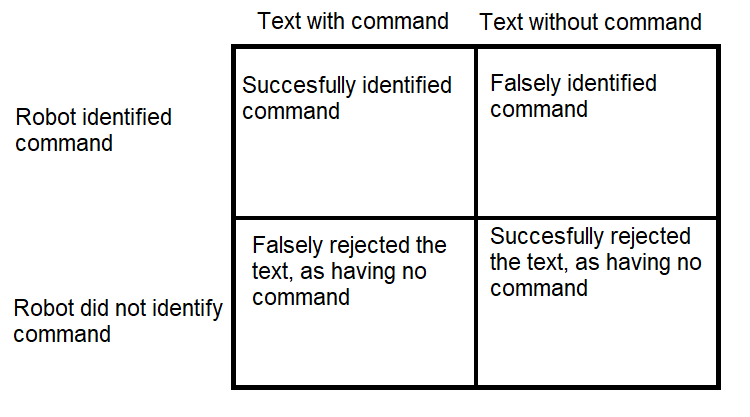
\includegraphics[width=15cm]{img/Confusion_table.png}
    \caption{Confusion table of the fail/pass criterias}
    \label{Confusion}
\end{figure}
Based on the event, that the input contains a command, and the 
robot succesfully detects it. 
Then the following robot movement will be used as 
an accuracy description, decribing the ratio between correctly interpreted movements, 
and falsely interpreted movements. 
For the neural network subsystem, another accuracy description is made, based 
on correct categorisations of POS tags. 
For the parser subsystem, another confusion table and accuracy description is created, 
having identical prerequisites for the evaluation of the whole system.
An interpretation of the evaluation of the parser subsystem, is observing it as 
an evaluation of the whole system, with the assumption, 
that the neural network gives ideal outputs.


